\chapter{Postdiction of Experimental Results}
\section{Coulumb Potential in RQM}
Coulomb's potential is different in that it describes a potential field extending radially outward from a source (charge), so using a spherical coordinates would be far simpler. In addition, Maxwell's equation inside the charged region becomes
\begin{equation}\partial^{\alpha} \partial_{\alpha} A^{\mu}=-e \bar{\psi} \gamma^{\mu} \psi\end{equation}
For N negatively charged fermions occupying the charged region, we can use a modified form:
\begin{equation}\partial^{\alpha} \partial_{\alpha} A^{\mu}=-N e \bar{\psi} \gamma^{\mu} \psi\end{equation}
\bluep{However, for the Coulomb potential this becomes simplified because that potential is measured in the region outside the charged region, where no charged fermion field $\psi$ exists. That is, the fermion field carrying the charge extends throughout the source particle/object to its surface, but no futher. Outside the surface, $\psi=0 .$ and that is our region of interest.}

So $\partial_{\alpha} \partial^{\alpha} A^{\mu}(x)=0$ governs in that region, and in spherical coordinates, we have
\begin{equation}\frac{\partial^{2}}{\partial t^{2}} A^{\mu}-\frac{1}{r} \frac{\partial^{2}}{\partial r^{2}}\left(r A^{\mu}\right)-\frac{1}{r^{2} \sin \theta} \frac{\partial}{\partial \theta}\left(\sin \theta \frac{\partial}{\partial \theta} A^{\mu}\right)-\frac{1}{r^{2} \sin ^{2} \theta \partial \phi^{2}} A^{\mu}=0\end{equation}
But since the field is symmetric spherically about the origin, where the charge is located, $A^{\mu}$ can only be a function of $r$ and $t .$ The Coulomb potential is static (not a function of $t$ ), so
\begin{equation}\frac{\partial^{2}}{\partial r^{2}}\left(r A^{\mu}\right)=0
\end{equation}
The general solution to this equation is $A^{\mu}=\varepsilon_{5}^{\mu} C / r+\varepsilon_{s}^{\mu} D,$ where $C$ and $D$ are constants. Physically, the potential must vanish at infinity, so $D=0$, and
\begin{equation}A^{\mu} \propto \frac{1}{r} \varepsilon_{s}^{\mu} \quad \text { or as column matrix, } \quad A^{\mu}=\left[\begin{array}{c}
A^{t} \\
A^{r} \\
A^{\theta} \\
A^{\phi}
\end{array}\right]=\frac{1}{r}\left[\begin{array}{c}
A_{0}^{t} \\
A_{0}^{r} \\
A_{0}^{\theta} \\
A_{0}^{\phi}
\end{array}\right]=\frac{1}{r}\left[\begin{array}{c}
\Phi_{0} \\
A_{0}^{1} \\
A_{0}^{2} \\
A_{0}^{3}
\end{array}\right]=\left[\begin{array}{c}
\Phi(r) \\
\mathbf{A}(r)
\end{array}\right]\end{equation}
From the physical symmetry, the 3 D yector potential can only have a radial direction, so it cannot bow have any component in the angular directions $\theta$ or $A_{0}^{\theta}=A_{0}^{\phi}=0 .$ Thus,
\begin{equation}
\mathbf{B}=\nabla \times \mathbf{A}=0
\end{equation}
and no magnetic field is product. To keep things simple, we can therefore just take $\mathcal{A}=0$, (i.e.,$A_0^{r}=0$ also) without loss of generality. From boundary conditions on the surface of the charged spherical source ($A^t=\Phi$ just on either side of the surface must be equal, though we won't go through the formal mathematics), we obtain the constant $A_0^t$. We then end up with the following well-known Coulomb potential in Heaviside-Lorentz units:
\begin{equation}A^{\mu}=\left[\begin{array}{c}
\Phi \\
0 \\
0 \\
0
\end{array}\right]=\left[\begin{array}{c}
-e N /(4 \pi r) \\
0 \\
0 \\
0
\end{array}\right]\end{equation}

\section{Coulomb Potential in QFT}
One could simply assume in QFT that the form of Coulomb potential is same as that in RQM, since we found throughout our development of both theories that they paralleled one another in terms of the governing equations and solution forms, and differed only in the interpretation of the solution coefficients as constants or operators. Here we present a derivation of the Coulomb potential from the perspective of QFT.
\subsection{Repulsive Coulomb Scattering Equivalence to Moller Scattering}
Repulsive Coulomb scattering can be represented by Moller scattering as shown in Fig. \ref{fig:coulomb-equiv}, where the source charge particle is spherical (has a radial distribution of its radiation)
\begin{figure}[H]
    \centering
\tikzset{every picture/.style={line width=0.75pt}} %set default line width to 0.75pt        

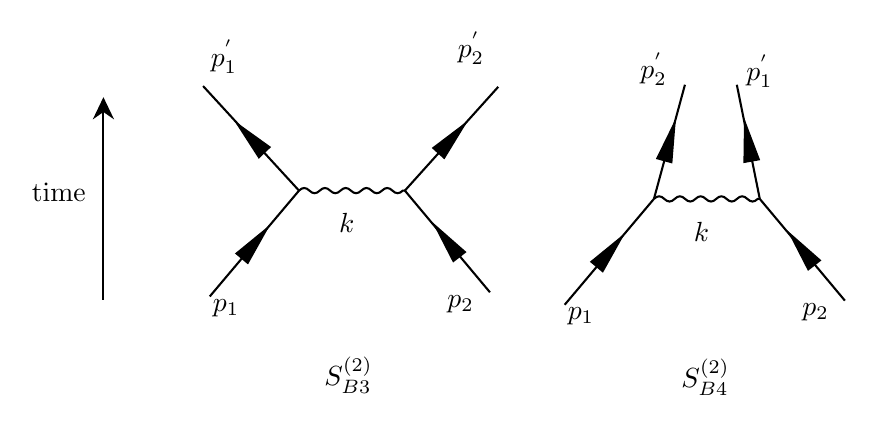
\begin{tikzpicture}[x=0.75pt,y=0.75pt,yscale=-1,xscale=1]
%uncomment if require: \path (0,300); %set diagram left start at 0, and has height of 300

%Straight Lines [id:da2660816173545789] 
\draw    (95,30.88) -- (141.23,81.27) ;
%Straight Lines [id:da5738036157098771] 
\draw    (141.23,81.27) -- (98.23,132.27) ;
%Straight Lines [id:da022647558542392976] 
\draw    (141.23,81.27) .. controls (142.9,79.6) and (144.56,79.6) .. (146.23,81.27) .. controls (147.9,82.94) and (149.56,82.94) .. (151.23,81.27) .. controls (152.9,79.6) and (154.56,79.6) .. (156.23,81.27) .. controls (157.9,82.94) and (159.56,82.94) .. (161.23,81.27) .. controls (162.9,79.6) and (164.56,79.6) .. (166.23,81.27) .. controls (167.9,82.94) and (169.56,82.94) .. (171.23,81.27) .. controls (172.9,79.6) and (174.56,79.6) .. (176.23,81.27) .. controls (177.9,82.94) and (179.56,82.94) .. (181.23,81.27) .. controls (182.9,79.6) and (184.56,79.6) .. (186.23,81.27) .. controls (187.9,82.94) and (189.56,82.94) .. (191.23,81.27) -- (192.23,81.27) -- (192.23,81.27) ;
%Straight Lines [id:da5942384241874531] 
\draw    (192.23,81.27) -- (233.23,130.27) ;
%Straight Lines [id:da2567536079404269] 
\draw    (192.23,81.27) -- (237.23,31.27) ;
%Shape: Triangle [id:dp9525733477827242] 
\draw  [fill={rgb, 255:red, 0; green, 0; blue, 0 }  ,fill opacity=1 ] (111.78,49.42) -- (126.99,60.32) -- (121.92,65.15) -- cycle ;
%Shape: Triangle [id:dp2592894694689559] 
\draw  [fill={rgb, 255:red, 0; green, 0; blue, 0 }  ,fill opacity=1 ] (125.64,99.72) -- (116.51,116.06) -- (111.15,111.56) -- cycle ;
%Shape: Triangle [id:dp8480575386658957] 
\draw  [fill={rgb, 255:red, 0; green, 0; blue, 0 }  ,fill opacity=1 ] (207.08,98.52) -- (221.14,110.87) -- (215.62,115.17) -- cycle ;
%Shape: Triangle [id:dp47648891796959525] 
\draw  [fill={rgb, 255:red, 0; green, 0; blue, 0 }  ,fill opacity=1 ] (220.9,49.45) -- (211.16,65.43) -- (205.97,60.74) -- cycle ;
%Straight Lines [id:da4906250054106407] 
\draw    (327.17,30.27) -- (312.23,85.27) ;
%Straight Lines [id:da9643681605781265] 
\draw    (312.23,85.27) -- (269.23,136.27) ;
%Straight Lines [id:da31569296455886353] 
\draw    (312.23,85.27) .. controls (313.9,83.6) and (315.56,83.6) .. (317.23,85.27) .. controls (318.9,86.94) and (320.56,86.94) .. (322.23,85.27) .. controls (323.9,83.6) and (325.56,83.6) .. (327.23,85.27) .. controls (328.9,86.94) and (330.56,86.94) .. (332.23,85.27) .. controls (333.9,83.6) and (335.56,83.6) .. (337.23,85.27) .. controls (338.9,86.94) and (340.56,86.94) .. (342.23,85.27) .. controls (343.9,83.6) and (345.56,83.6) .. (347.23,85.27) .. controls (348.9,86.94) and (350.56,86.94) .. (352.23,85.27) .. controls (353.9,83.6) and (355.56,83.6) .. (357.23,85.27) .. controls (358.9,86.94) and (360.56,86.94) .. (362.23,85.27) -- (363.23,85.27) -- (363.23,85.27) ;
%Straight Lines [id:da8747821979538987] 
\draw    (363.23,85.27) -- (404.23,134.27) ;
%Straight Lines [id:da2726790256119972] 
\draw    (363.23,85.27) -- (352.17,30.27) ;
%Shape: Triangle [id:dp4558179765191268] 
\draw  [fill={rgb, 255:red, 0; green, 0; blue, 0 }  ,fill opacity=1 ] (322.13,48.9) -- (320.64,67.56) -- (313.89,65.7) -- cycle ;
%Shape: Triangle [id:dp6395959312057592] 
\draw  [fill={rgb, 255:red, 0; green, 0; blue, 0 }  ,fill opacity=1 ] (296.64,103.72) -- (287.51,120.06) -- (282.15,115.56) -- cycle ;
%Shape: Triangle [id:dp13394205394546932] 
\draw  [fill={rgb, 255:red, 0; green, 0; blue, 0 }  ,fill opacity=1 ] (378.08,102.52) -- (392.14,114.87) -- (386.62,119.17) -- cycle ;
%Shape: Triangle [id:dp17889896090170887] 
\draw  [fill={rgb, 255:red, 0; green, 0; blue, 0 }  ,fill opacity=1 ] (356.11,48.71) -- (362.74,66.21) -- (355.84,67.43) -- cycle ;
%Straight Lines [id:da41746806197259423] 
\draw    (47,133.88) -- (47,39.27) ;
\draw [shift={(47,36.27)}, rotate = 450] [fill={rgb, 255:red, 0; green, 0; blue, 0 }  ][line width=0.08]  [draw opacity=0] (10.72,-5.15) -- (0,0) -- (10.72,5.15) -- (7.12,0) -- cycle    ;

% Text Node
\draw (98.23,132.27) node [anchor=north west][inner sep=0.75pt]    {$p_{1}$};
% Text Node
\draw (211.23,130.27) node [anchor=north west][inner sep=0.75pt]    {$p_{2}$};
% Text Node
\draw (97.23,7.27) node [anchor=north west][inner sep=0.75pt]    {$p^{'}_{1}$};
% Text Node
\draw (216.23,3.27) node [anchor=north west][inner sep=0.75pt]    {$p^{'}_{2}$};
% Text Node
\draw (159,90.88) node [anchor=north west][inner sep=0.75pt]    {$k$};
% Text Node
\draw (269.23,136.27) node [anchor=north west][inner sep=0.75pt]    {$p_{1}$};
% Text Node
\draw (382.23,134.27) node [anchor=north west][inner sep=0.75pt]    {$p_{2}$};
% Text Node
\draw (355.23,14.27) node [anchor=north west][inner sep=0.75pt]    {$p^{'}_{1}$};
% Text Node
\draw (304.23,13.27) node [anchor=north west][inner sep=0.75pt]    {$p^{'}_{2}$};
% Text Node
\draw (330,94.88) node [anchor=north west][inner sep=0.75pt]    {$k$};
% Text Node
\draw (11,75.88) node [anchor=north west][inner sep=0.75pt]   [align=left] {time};
% Text Node
\draw (152,159.88) node [anchor=north west][inner sep=0.75pt]    {$S^{( 2)}_{B3}$};
% Text Node
\draw (324,160.88) node [anchor=north west][inner sep=0.75pt]    {$S^{( 2)}_{B4}$};


\end{tikzpicture}

    \caption{Moller Scattering}
    \label{fig:coulomb-equiv}
\end{figure}

\bluep{If the incoming particles in Fig. \ref{fig:coulomb-equiv} are indistinguishable, such as two electrons, we need to include both diagrams to determine the amplitude.} But, if they are distinguishable, such as an electron and a muon, then we only need to consider the LH diagram, (Because there is no indeterminancy in which orlginal particle mutated into which final particle.) Further, the classical Coulomb potential is always between macro (distinguishable) objects So, to make things simpler, we will assume the particles are distinguishable and examine the transition amplitude for only the LH diagram in the figure.

We also assume non-relativistic speeds of our incoming and outgoing particles, as that is typically the case for Coulomb scattering. One can \bluep{think of the particle labeled 1 as the source, whose radiated virtual particle affects the particle labeled 2}.

\subsection{Relations We Need}
Recall that the Fourier transforms of each other, $g(k)$ and $f(x)$, are defined as
\begin{equation}g(k)=\int_{-\infty}^{+\infty} f(x) e^{-i k x} d x \quad \Leftrightarrow \quad f(x)=\frac{1}{2 \pi} \int_{-\infty}^{+\infty} g(k) e^{i k \pi} d k\end{equation}
From almost any table of Fourier transform pairs, we can get the following relations.
\begin{equation}\frac{1}{k} \quad \Leftrightarrow \quad \frac{i}{2} \operatorname{sgn} x\left(\frac{i}{2} \text { for } x>0 \quad-\frac{i}{2} \text { for } x<0\right)\end{equation}
\begin{equation}\frac{1}{k^{2}} \quad \Leftrightarrow \quad-\frac{1}{2}|x|\end{equation}
In deriving the Coulomb potential using QFT under non-relativisitic conditions, we will need to refer to a result from NRQM, namely the scattering of two charged particles from one another. In NRQM, actually, the charge on one particle is assumed to \redp{provide a potential $V(\mathcal{x})$ to which the other particle wave function responds.} So we consider the behavior of one wave function in a given potential.

To get the NRQM transition amplitude, one usually employs the Born approximation, which assumes the incoming wave remains undistorted even within the scattering region. In fact, it is distorted, but modestly so, and the approximation gives results quite close to experiment. Thus, (with $V$ the volume of the interaction, and $\tilde{V}(\mathbf{k})$ the Fourier transform of $V(\mathbf{x})$ ) the Born approximation scattering amplitude in NRQM in terms of a single particle in a potential $V(x)$ is
\begin{equation}S_{f i}=\frac{i}{V} \tilde{V}(\mathbf{k}) 2 \pi \delta\left(E_{f}-E_{i}\right) \quad \text { where } \mathbf{k}=\mathbf{p}_{i}-\mathbf{p}_{f}
\label{NRQM-transition-amplitude}
\end{equation}
This result extends to the case where two particles interact, such as in Fig. \ref{fig:coulomb-equiv} where $\tilde{V}(\mathbf{k})$ is the Fourier transform of $V(x)$, the potential field one particle feels due to the other.
\begin{equation}S_{f i}=\frac{i}{V^{2}} \tilde{V}(\mathbf{k})(2 \pi)^{4} \delta^{(4)}\left(p_{f}-p_{i}\right) \text { where } \mathbf{k}=\mathbf{p}_{i}-\mathbf{p}_{f}\end{equation}
\subsection{A Detour for the Planar Potential}
We have been using plane wave fields and particles to develop our theory. So it will be easier if we investigate plane wave potentials that arise from plane wave fields/particles first. Thus, we now
i) derive the transition amplitude for plane waves (meaning a planar charge distribution) in Moller scattering using QFT at non-relativistic speeds, then

ii) compare the result with (\ref{NRQM-transition-amplitude}) (b) to deduce the potential in 3 -momentum space, and finally,

iii) Fourier transform the result to obtain that potential in 3 D physical space

Using Feynman's rule, we have
\begin{equation}\begin{array}{l}
S_{\text {difiting }}=\left(\prod_{p}^{\text {allexternal }} \sqrt{\frac{m}{V E_{p}}}\right)(2 \pi)^{4} \delta^{(4)}\left(p_{1}^{\prime}+p_{2}^{\prime}-p_{1}-p_{2}\right) \mathcal{M}_{B 3}^{(2)} \\
\mathcal{M}_{B 3}^{(2)}=e^{2} \bar{u}_{r1^{\prime}}\left(\mathbf{p}_{1}^{\prime}\right) \gamma^{\mu} u_{r1}\left(\mathbf{p}_{1}\right) i D_{F \mu \nu}\left(k=p_{1}-p_{1}^{\prime}\right) \bar{u}_{r_{2}^{\prime}}\left(\mathbf{p}_{2}^{\prime}\right) \gamma^{\nu} u_{r2}\left(\mathbf{p}_{2}\right) 
\end{array}\end{equation}
where a subscript such as $r_{2}$ means the $r$ spin state $\left(r_{2}=1,2\right)$ of particle \#2. We will be considering non-relativistic speeds, where $E \approx m$ and $|p|<<m$ So our spinors will, to good approximation, become (with subscripts here referring to the spin state $r$ )
$$u_{r=1}(\mathbf{p})=\sqrt{\frac{E+m}{2 m}}\left(\begin{array}{c}
1 \\
0 \\
\frac{p^{3}}{E+m} \\
\frac{p^{1}+i p^{2}}{E+m}
\end{array}\right) \Rightarrow\left(\begin{array}{l}
1 \\
0 \\
0 \\
0
\end{array}\right)$$
$$u_{r=2}(\mathbf{p})=\sqrt{\frac{E+m}{2 m}}\left(\begin{array}{c}
0 \\
1 \\
\frac{p^{1}-i p^{2}}{E+m} \\
\frac{-p^{3}}{E+m}
\end{array}\right) \Rightarrow\left(\begin{array}{l}
0 \\
1 \\
0 \\
0
\end{array}\right)$$
For non-relativistic conditions, spinors become effectively independent of $\mathbf{p}$,so
$$u_{r_{1}=1}\left(\mathbf{p}_{1}\right) \approx u_{r_{2}=1}\left(\mathbf{p}_{2}\right) \quad u_{r_{1}=2}\left(\mathbf{p}_{1}\right) \approx u_{r_{2}=2}\left(\mathbf{p}_{2}\right)$$
and
$$\begin{aligned}
&\vec{u}_{n}=u\left(\mathbf{p}_{1}^{\prime}\right)=u_{n^{2}=1}^{\dagger}\left(\mathbf{p}_{1}^{\prime}\right) \gamma^{0} \Rightarrow\left(\begin{array}{llll}
1 & 0 & 0 & 0
\end{array}\right)\\
&\vec{u}_{n}=2\left(p_{1}^{\prime}\right)=u_{r_{1}^{\prime}=2}^{\dagger}\left(p_{1}^{\prime}\right) \gamma^{0} \Rightarrow\left(\begin{array}{llll}
0 & 1 & 0 & 0
\end{array}\right)
\end{aligned}$$
$$\begin{array}{l}
\bar{u}_{2}^{\prime}=1\left(\mathrm{p}_{2}^{\prime}\right)=u_{2}^{\dagger}+\left(\mathrm{p}_{2}^{\prime}\right) \gamma^{0} \Rightarrow(1 \quad 0 \quad 0 \quad 0) \\
\bar{u}_{r_{2}^{\prime}=2}\left(\mathrm{p}_{2}^{\prime}\right)=u_{r_{2}^{\prime}=2}^{\dagger}\left(\mathrm{p}_{2}^{\prime}\right) \gamma^{0} \Rightarrow(0,1,0 \quad 0)
\end{array}$$
So for non-relativisitc conditions, the feynman amplitude becomes,where we assume the case where $r_1=1$ and $r_2=1$,
$$\mathcal{M}_{B 3}^{(2)}=e^{2} \bar{u}_{r_{1}^{\prime}}\left(\mathbf{p}_{1}^{\prime}\right)\left[\begin{array}{ll}
1 & \\
& 1
\end{array}\right]\left[\begin{array}{l}
1 \\
0
\end{array}\right] \frac{-i g_{00}}{k^{2}+i \varepsilon} \bar{u}_{r_{2}^{\prime}\left(\mathbf{p}_{2}^{\prime}\right)}\left[\begin{array}{ll}
1 & \\
& 1
\end{array}\right]\left[\begin{array}{l}
1 \\
0
\end{array}\right]$$
\textbf{This is enly non-zero if the adjoint spinors both equal ( 1 0). As an aside, this means the spins of the incoming and outgoing particles each remain unchanged.}

Additionally, for elastic scattering in the center of mass (COM) system for two particles of equal mass, the two particles start with the same speed and end with the same speed, but they exchange velocities (directions). Thus, neither changes its kinetic energy, and thus, \textbf{no energy is carried by the virtual particle from one real particle to the another}. However, there is 3 -momentum exchange because the drection of each purticle's velocity clanges. Hence $k^{2}=-\mathbf{k}^{2}$($\omega=0$) in the propagator. So
\begin{equation}M_{B 3}^{(2)}=-i e^{2} \frac{1}{-\mathbf{k}^{2}+i \varepsilon}\end{equation}
And the treansition amplitude is
\begin{equation}S_{\text {Moller}}=i e^{2} \frac{1}{V^{2}}(2 \pi)^{4} \delta^{(4)}\left(p_{1}^{\prime}+p_{2}^{\prime}-p_{1}-p_{2}\right) \frac{1}{\mathbf{k}^{2}}\end{equation}
Comparing the eqn. above with (\ref{NRQM-transition-amplitude}), we conclude that
\begin{equation}\tilde{V}(\mathrm{k})=\frac{e^{2}}{\mathbf{k}^{2}}\end{equation}
To find the potential in physical space, consider $k$ in the $x^1$ direction and we have
\begin{equation}V\left(x^{1}\right)=-\frac{1}{2} e^{2}\left|x^{1}\right| \quad=-\frac{1}{2} e^{2} x^{1}\end{equation}
\subsection{Repulsive Coulomb Potential via QFT}
We start with plane wave derivation, deduce the 3-momentum space potential $\tilde{V}(\mathcal{k})$, and in Fourier transforming that, change from Cartesian to spherical 3D coordiantes. To this end, we can use the same low velocity Moller scattering amplitude that we already derived. From that and (\ref{NRQM-transition-amplitude}) we get the same momentum space potential. The only issue remaining is to transform that to position space, expressed in spherical coordinates. Start with
\begin{equation}V(\mathrm{x})=\frac{1}{(2 \pi)^{3}} \int \tilde{V}(\mathrm{k}) e^{i \mathrm{k} \cdot \mathrm{x}} d^{3} k=\frac{1}{(2 \pi)^{3}} \int_{-\infty}^{\infty} \frac{e^{2}}{\mathrm{k}^{2}} e^{i \mathrm{k} \cdot \mathrm{x}} d^{3} k\end{equation}
and note that for spherical coordinates $r, \theta, \phi$ in $\mathrm{k}$ space we can align the $k^{3}$ axis (the $\theta=0$ direction) with the direction of the position vector $x$. With that alignment and with x representing any point in position space, $\mathbf{k} \cdot \mathbf{x}=|\mathbf{k} \| \mathbf{x}| \cos \theta,$ where we now use the symbol $k$ as $=|\mathbf{k}|$ (usually it has been shorthand for $k^{\prime \prime}$ ) and $|x|=r$, for the remainder of this section. Thus, $k \cdot x=k r \cos \theta$ and $k^{2}=k^{2}$ for the temporary notation.

The differential volume element $d^{3} k$ in spherical coordinates in $\mathbf{k}$ space is $k^{2}$ sin $\theta d \theta d \phi d k$. Given this, 
\begin{equation}V(r)=\frac{1}{(2 \pi)^{3}} \int_{0}^{\infty} \int_{0}^{\pi} \int_{0}^{2 \pi} \frac{e^{2}}{k^{2}} e^{i k r\cos \theta} k^{2} \underbrace{\sin \theta d \theta}_{-d(\cos \theta)} d \phi d k=\frac{-e^{2}}{(2 \pi)^{3}} 2 \pi \int_{0}^{\infty} \int_{0}^{\pi} e^{i k r \cos \theta} d \underbrace{(\cos \theta)}_{\text {take as } u} d k\end{equation}
$$=\frac{e^{2}}{(2 \pi)^{2}} \int_{0}^{\infty}\left(\frac{e^{i k r}-e^{-i k r}}{i k r}\right) d k$$
The last part can then be re-expressed as an integral from - $\infty$ to $+\infty$, as follows (where in going to the last term in the first row below, we substitute variable $k \rightarrow-k$ ).
$$V(r)=\frac{e^{2}}{(2 \pi)^{2}}\left(\int_{0}^{\infty}\left(\frac{e^{i kr}}{i k r}\right) d k-\int_{0}^{\infty}\left(\frac{e^{-i k r}}{i k r}\right) d k\right)=\frac{e^{2}}{(2 \pi)^{2}}\left(\int_{0}^{\infty}\left(\frac{e^{i k r}}{i k r}\right)(d k)-\int_{0}^{-\infty}\left(\frac{e^{-i(-k) r}}{i(-k) r}\right)(-d k)\right)$$
$$=\frac{e^{2}}{(2 \pi)^{2}}\left(\int_{0}^{\infty}\left(\frac{e^{i t \tau}}{i k r}\right)(d k)+\int_{-\infty}^{0}\left(\frac{e^{i k r}}{i k r}\right) d k\right)$$
$$=\frac{e^{2}}{(2 \pi)^{2}} \int_{-\infty}^{\infty} \frac{e^{i k r}}{i k r} d k=\frac{e^{2}}{i r 2 \pi} \underbrace{\frac{1}{2 \pi} \int_{-\infty}^{\infty} \frac{e^{i k r}}{k} d k}_{=i / 2 \text { from table }}$$
thus
\begin{equation}V(r)=\frac{e^{2}}{4 \pi r}\end{equation}

\subsection{Attractive Coulomb Potential via QFT}
For oppositely charged particle, we have Bhabha scattering (without annihilation) instead of Moller. Its transition amplitude is
\begin{equation}S_{\text {Bhabha }}^{(2)}=S_{B 2}^{(2)}=\left(\prod_{\text {no annih }}^{\text {allextemal }} \sqrt{\frac{m}{V E_{\mathrm{p}}}}\right)(2 \pi)^{4} \delta^{(4)}\left(p_{1}^{\prime}+p_{2}^{\prime}-\left(p_{1}+p_{2}\right)\right) \mathcal{M}_{B 2}^{(2)}
\label{attractive-coulomb}
\end{equation}
where
\begin{equation}\mathcal{M}_{B_{2} 2}^{(2)}=-e^{2} \bar{v}_{r1}\left(\mathbf{p}_{1}\right) \gamma^{\mu} v_{r_1'} \cdot\left(\mathbf{p}_{1}^{\prime}\right) i D_{F \mu \nu}\left(p_{1}-p_{1}^{\prime}\right) \bar{u}_{r_{2}}^{\prime}\left(\mathbf{p}_{2}^{\prime}\right) \gamma^{v} u_{r2}\left(\mathbf{p}_{2}\right)\end{equation}
So, (\ref{attractive-coulomb}) is similar to Moller except for the sign as we have to maintain normal ordering. At non-relativistic speeds, we have
$$v_{r=1}(\mathbf{p})=\sqrt{\frac{E+m}{2 m}}\left(\begin{array}{c}
\frac{p^{3}}{E+m} \\
\frac{p^{1}+i p^{2}}{E+m} \\
1 \\
0
\end{array}\right) \Rightarrow\left(\begin{array}{l}
0 \\
0 \\
1 \\
0
\end{array}\right)$$
$$v_{r=2}(\mathbf{p})=\sqrt{\frac{E+m}{2 m}}\left(\begin{array}{c}
\frac{p^{1}-i p^{2}}{E+m} \\
\frac{-p^{3}}{E+m} \\
0 \\
1
\end{array}\right) \Rightarrow\left(\begin{array}{l}
0 \\
0 \\
0 \\
1
\end{array}\right)$$
And we can show that 
\begin{equation}\mathcal{M}_{B 2}^{(2)}=i e^{2} \frac{1}{-\mathbf{k}^{2}+i \varepsilon}\end{equation}
at low speed. And
\begin{equation}\tilde{V}(\mathrm{k})=-\frac{e^{2}}{\mathbf{k}^{2}}\end{equation}
\begin{equation}V(r)=-\frac{e^{2}}{4 \pi r}\end{equation}